\section{Data}
\label{sec:data}

We use Python \citep{python3} to analyze S\&P500 price data from Yahoo Finance \citep{yahoo_finance_gspc} and the Fama-French 3-factor data library \citep{french_website}.
Yahoo finance provides daily price data of the S\&P500 which we resample to monthly returns for the period 1950 - 2024. We get monthly log returns by taking the
difference of the log of the adjusted close price of the S\&P500 for each month (Figure~\ref{fig:sp500-returns}). Our timeseries starts in 1950
based on the premise that the market prior to this was not as sophisticated prior to this date,
 and is not illustrative for the purposes of this analysis of market efficiency and value spreads \citep{asness_2024}.

\begin{figure}[h!]
    \centering
    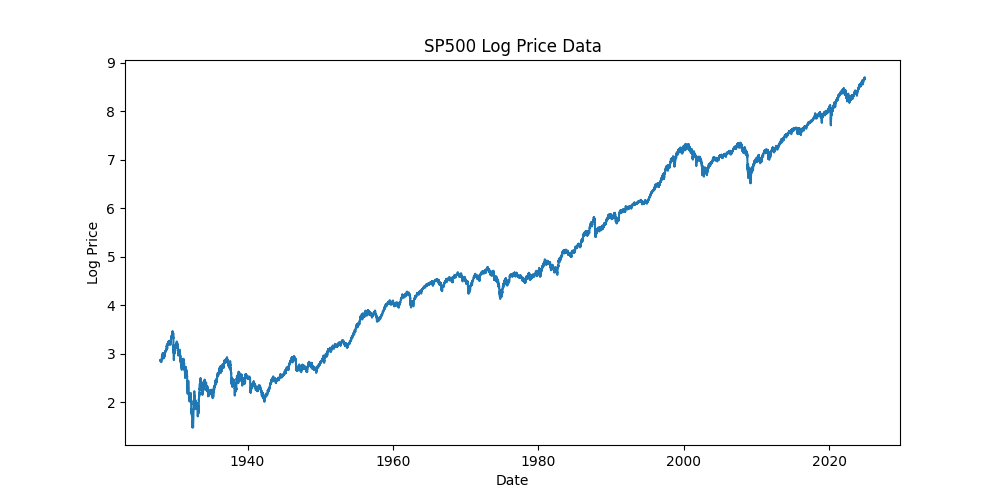
\includegraphics[width=1\textwidth]{../data/03-analysis_data_visuals/sp500_log_price.png}
    \caption{The S\&P500 timeseries 1950 - 2024.}
    \label{fig:sp500-returns}
\end{figure}

\subsection{Cumulative Log Returns}
\begin{table}[ht]
\centering
\resizebox{\textwidth}{!}{%
\begin{tabular}{lrrrrrrr}
\toprule
Date & Cum Log Return 1 & Cum Log Return 2 & Cum Log Return 3 & ... & Cum Log Return 34 & Cum Log Return 35 & Cum Log Return 36 \\
\midrule
1950-01-01 & 0.0154 & 0.0253 & 0.0293 & ... & 0.379 & 0.424 & 0.459 \\
1950-02-01 & 0.0100 & 0.0140 & 0.0520 & ... & 0.409 & 0.444 & 0.436 \\
1950-03-01 & 0.00412 & 0.0421 & 0.0867 & ... & 0.434 & 0.427 & 0.408 \\
1950-04-01 & 0.0380 & 0.0827 & 0.0229 & ... & 0.422 & 0.404 & 0.380 \\
1950-05-01 & 0.0446 & -0.0151 & -0.00672 & ... & 0.366 & 0.342 & 0.315 \\
\bottomrule
\end{tabular}
}
\caption{Cumulative log S\&P500 return periods for each month. Each column represents the cumulative log return for a given period starting 
at the row index, and ending $t$ months ahead.}
\label{tab:cumulative-log-returns}
\end{table}

The unbiasedness regression require windows of cumulative returns. For any month $t$, we get every forward month's returns up to T months.
By taking expanding window sums of the columns of log returns, we get a cumulative log returns matrix (Table~\ref{tab:cumulative-log-returns}).

\subsection{The Value Spread}

The value spread is the ratio of average book-to-market of the most expensive 30\% portfolio to the price-to-book of the portfolio of the cheapest 30\% of stock portfolio, as per \citet{fama_french_1993}.
To construct this measure we use Kenneth French's data library \citep{french_website}. 
Using French's 3x2 sort on book-to-market and market equity, we get the monthly market value weighted average of the book-to-value of the portfolio of the 30\% most expensive large-cap stocks and the portfolio of the 30\% cheapest large-cap stocks. The value spread is the ratio of these two averages.
It represents how much more expensive the expensive stocks are compared to the cheap stocks (Figure~\ref{fig:value_spread}).

\begin{figure}[h!]
    \centering
    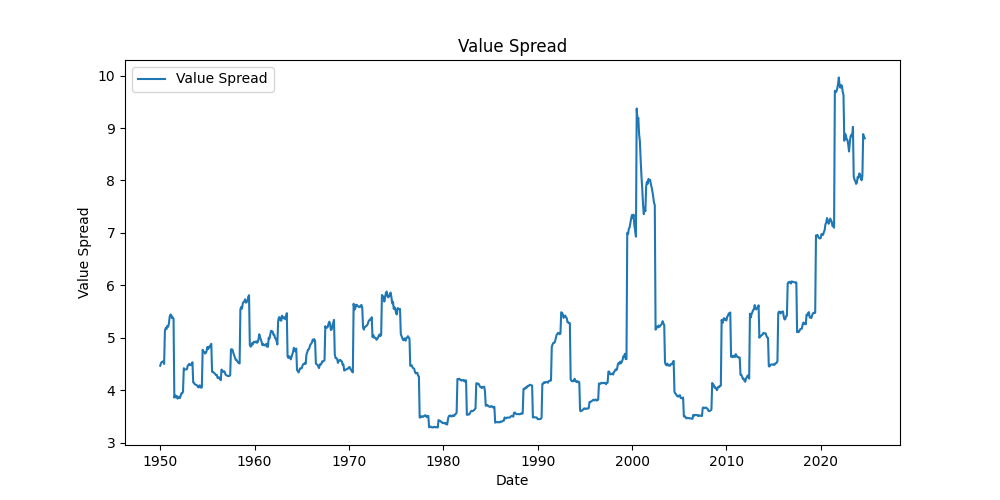
\includegraphics[width=1\textwidth]{../figs/Value Spread.png}
    \caption{The value spread timeseries 1950 - 2024. \citet{asness_2024} argues the widening spread in the last decade is due to increasing market inefficiency.}
    \label{fig:value_spread}
\end{figure}